\documentclass[11pt]{article}

\usepackage[T1]{fontenc}
\usepackage[utf8]{inputenc}
\usepackage{lmodern}
\usepackage{amsmath,amssymb}
\usepackage{graphicx}
\usepackage{geometry}
\usepackage{hyperref}

\geometry{margin=1in}

\title{Numerical Workflow for Surface-Electrode Ion Trap Design}
\author{Dan Hawkley}
\date{}

\begin{document}

\maketitle

\section*{Overview}

This work presents a numerical workflow for the design and optimization of surface-electrode ion traps. The pipeline integrates electrostatic modeling, parameter sweeps, and physical scaling to produce hardware-relevant trap characteristics.

\begin{center}
geometry $\rightarrow$ Laplace solve $\rightarrow$ electric field $\rightarrow$ pseudopotential $\rightarrow$ trap detection $\rightarrow$ optimization $\rightarrow$ physical metrics
\end{center}

Outputs include trap height ($\mu$m), pseudopotential scale (eV), and secular frequencies (MHz).

\section*{Method}

\subsection*{Electrostatics}

We solve:
\[
\nabla^2 V = 0
\]

\subsection*{Field}

\[
\mathbf{E} = -\nabla V
\]

\subsection*{Pseudopotential}

\[
\Phi_{\mathrm{pseudo}} = \frac{q^2 |\mathbf{E}|^2}{4 m \Omega^2}
\]

\subsection*{Trap Condition}

\[
\lambda_i > 0
\]

\subsection*{Objective}

\[
\text{score} = \frac{\text{trap strength}}{\text{trap height}^2}
\]

\section*{Results}

The optimization produces a physically consistent trapping configuration. The pseudopotential map (Fig. 1) shows a stable minimum above the electrode surface.

\begin{itemize}
\item Trap height: $\sim 30\,\mu\mathrm{m}$
\item Secular frequency: $\sim 1$--$2\,\mathrm{MHz}$
\item Stable quadratic confinement near the trap point
\end{itemize}

\begin{figure}[h]
\centering
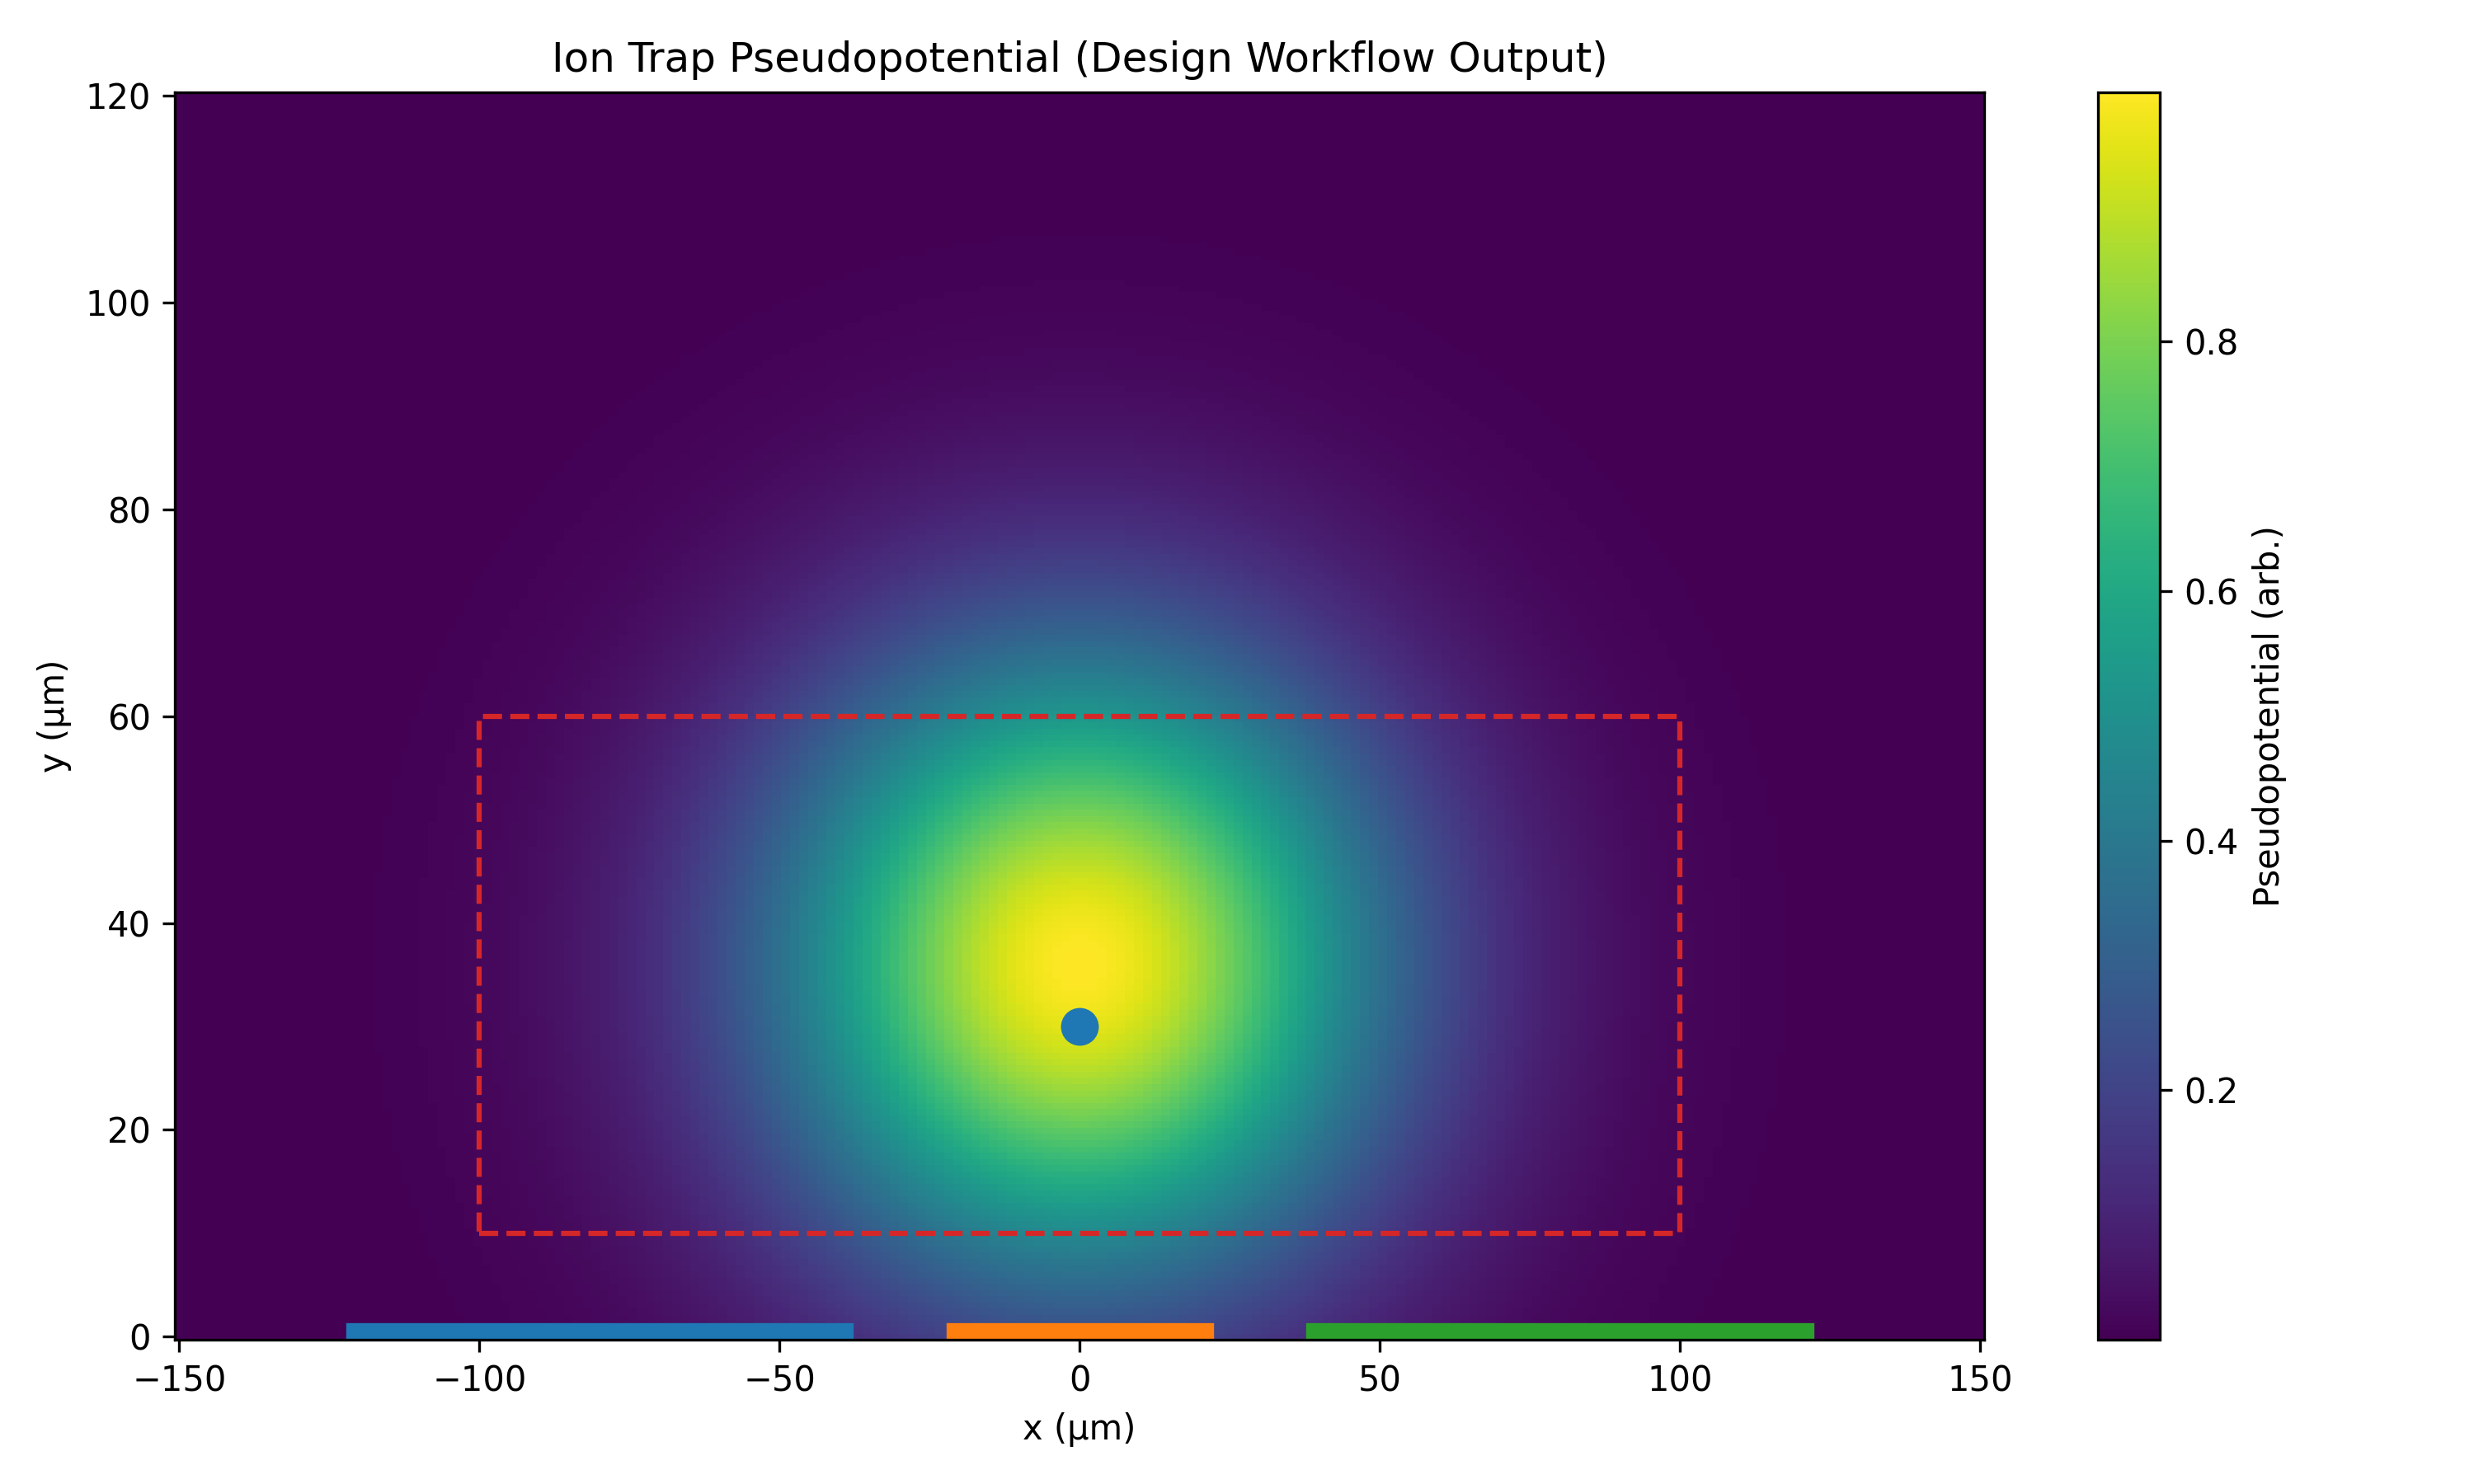
\includegraphics[width=0.85\textwidth]{hero_figure.png}
\caption{RF pseudopotential map showing electrode geometry (bottom), optimized trap location (blue point), and search window (dashed). The trap forms as a stable minimum above the RF electrode.}
\end{figure}

\section*{Interpretation}

The results reflect expected surface-trap behavior:

\begin{itemize}
\item Smaller electrode spacing increases electric field gradients and confinement strength
\item Larger geometries raise the trap height but reduce curvature
\item Optimal designs balance confinement strength against practical trapping distance
\end{itemize}

The objective function
\[
\text{score} = \frac{\text{trap strength}}{\text{trap height}^2}
\]
encodes this tradeoff, favoring strong confinement while penalizing traps that form too far from the surface.

\section*{Conclusion}

This workflow provides:

\begin{itemize}
\item Electrostatic modeling
\item Multi-parameter optimization
\item Curvature-based trap validation
\item Conversion to physical units
\end{itemize}

It mirrors early-stage trapped-ion design and produces realistic trap metrics.

\vspace{0.5em}
\noindent
\textbf{Code:} \url{https://github.com/thinkthoughts/ion-trap-parameter-lab}

\end{document}
